% Chapter 8 -- Claim: Value Beats Growth
% Requires: amsmath, amssymb, booktabs, array, tabularx, graphicx, tcolorbox (breakable, skins), hyperref or url.
% Defines the callout box only if the preamble has not.
\providecolor{fenavy}{HTML}{1B2A6B}
\providecolor{feshade}{HTML}{F3F5FA}
\makeatletter
\@ifundefined{callout}{%
  \newtcolorbox{callout}{breakable, enhanced,
    colback=white, colframe=gray!70, boxrule=0.5pt, arc=1mm,
    borderline west={2.5pt}{0pt}{gray!70},
    left=8pt, right=8pt, top=4pt, bottom=4pt}%
}{}
\makeatother

\chapter{Claim: Value Beats Growth}
\label{ch:08}

Buying what is cheap is the oldest idea in investing. Benjamin Graham taught it in the 1930s (Graham and Dodd 1934), Warren Buffett built a fortune on a refined version of it, and in the early 1990s academic finance gave it a name, a number and a factor: the value premium, measured by HML. For three decades afterward, a tilt toward value stocks was one of the most widely recommended departures from the market portfolio, built into index funds, smart-beta products and the asset allocations of large institutions.

Then, from about 2007, value stopped working in the United States. For more than a decade expensive growth stocks beat cheap value stocks by a wide margin, and the debate turned from why value works to whether it ever did, whether it had been arbitraged away, or whether accounting had changed what ``cheap'' means.

This chapter puts the claim on trial with a century of U.S. data, other measures of cheapness, other countries and the investor's own question: even if the premium is real, could you have held on long enough to collect it?

By the end of the chapter you will be able to:

\begin{itemize}
  \item compute book-to-market and other valuation ratios, and explain why intangible investment distorts book value;
  \item explain what an anomaly is, and how portfolio sorts and long--short factors are built;
  \item construct HML from the six size and book-to-market portfolios;
  \item compare the risk and mispricing explanations of the value premium;
  \item state the claim that value beats growth in a form that can fail, and test it over time, across measures, among large stocks, abroad and after costs;
  \item size a value tilt you could hold through a decade of underperformance.
\end{itemize}

\section{Foundations: accounting value, anomalies and factor portfolios}
\label{sec:08-foundations}

\textbf{Book value and market value.} A firm's \textbf{book value of equity} is an accounting figure from its \textbf{balance sheet}, the statement of what a firm owns and owes: total assets minus total liabilities, built mainly from the historical cost of what the firm has invested, less \textbf{depreciation}, the gradual write-down of assets as they wear out. Its \textbf{market value of equity} is the share price times shares outstanding: what investors think the firm's future cash flows are worth today. The ratio of the two, \textbf{book-to-market} (or its inverse, price-to-book), compares what the firm has put in with what the market expects it to earn.

Accounting rules record spending on factories and equipment as assets, but treat most spending on research, software, brands and training as expenses that reduce earnings and never appear on the balance sheet. Firms that invest mainly in such \textbf{intangible} assets therefore tend to have low book values relative to their market values (Figure~\ref{fig:08-book}).

\textbf{Other valuation ratios.} Each of these measures how much the investor gets per dollar paid:

\begin{itemize}
  \item \textbf{earnings-to-price} (the inverse of the P/E ratio) compares annual profits with the share price;
  \item \textbf{cash flow-to-price} uses earnings plus depreciation and other non-cash charges;
  \item \textbf{dividend yield} uses dividends paid.
\end{itemize}

Stocks high on these ratios are called \textbf{value} stocks, those low on them \textbf{growth} stocks.

\textbf{The CAPM and its failures.} The capital asset pricing model says that a stock's expected excess return is its market beta times the market's expected excess return (Chapter 3). A stock's \textbf{alpha} is the part of its average return the model does not explain. From the late 1970s, researchers found that stocks with high earnings-to-price or book-to-market ratios had positive alphas: they earned more than their betas justified. These became known as \textbf{anomalies}, patterns the CAPM could not explain.

\textbf{Portfolio sorts.} The standard empirical method for studying a characteristic like book-to-market is a \textbf{portfolio sort}:

\begin{enumerate}
  \item at regular intervals, rank all stocks on the characteristic;
  \item group them into portfolios: deciles (ten groups), quintiles (five) or the 30/40/30 split used for HML;
  \item hold each portfolio for a period, and record its return.
\end{enumerate}

A \textbf{long--short} or \textbf{high-minus-low} portfolio buys the top group and sells the bottom one. If the characteristic is related to expected returns, the long--short portfolio will earn a positive average return.

\textbf{Factors and factor models.} When a long--short portfolio captures a pattern shared by many stocks, it can serve as a \textbf{factor} in a model of expected returns. The Fama--French three-factor model explains expected excess returns with the market, a size factor (SMB) and a value factor (HML). A stock's or fund's \textbf{loadings} on these factors, estimated by regression, describe its style; its alpha relative to the model measures what the factors do not explain.

\textbf{Worked example.} A company has book equity of \$2 billion and 100 million shares trading at \$50, a market value of \$5 billion. Its book-to-market ratio is $2/5 = 0.4$ and its price-to-book ratio 2.5. If it had spent \$1 billion on research over the past five years that accounting treated as expenses, and that spending were instead counted as an asset, its adjusted book-to-market would be closer to $3/5 = 0.6$.

\begin{figure}[htbp]
\centering
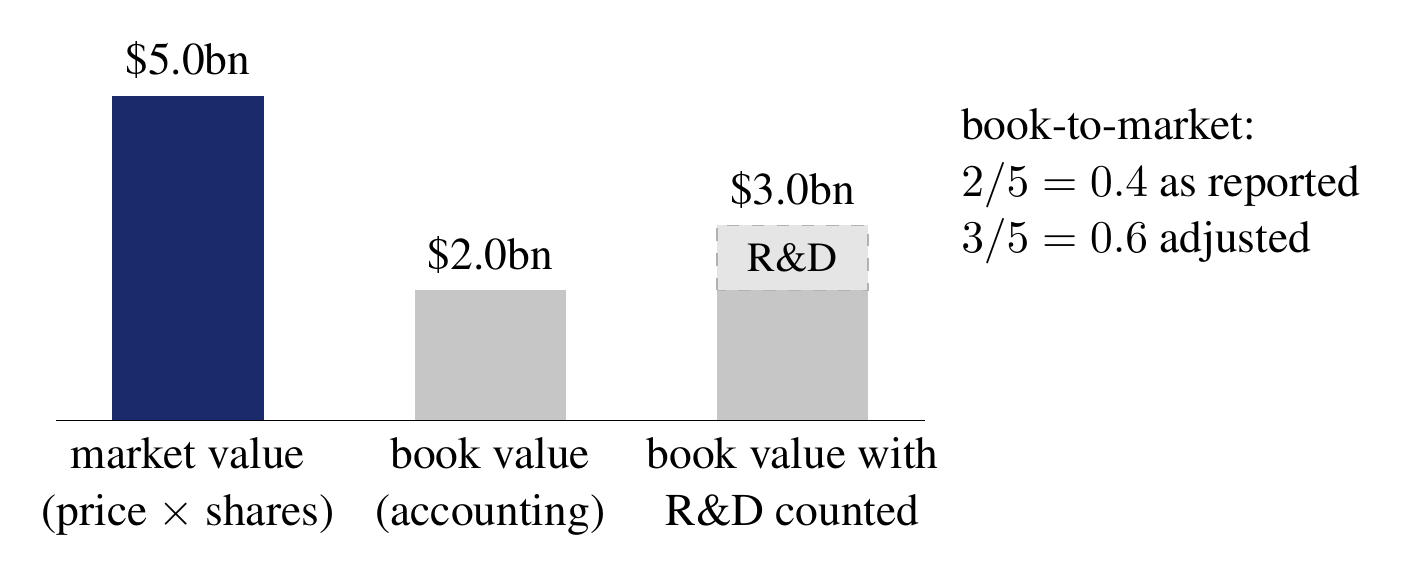
\includegraphics[width=0.85\linewidth]{images/fig08-1-book-market.png}
\caption{Book value, market value and intangibles, from the worked example. Counting past research spending as an asset raises book value from \$2 billion to \$3 billion and book-to-market from 0.4 to 0.6, moving the firm toward the value end of a sort.}
\label{fig:08-book}
\end{figure}

\textbf{Further reading.} Bodie, Kane and Marcus, \emph{Investments}, chapters on financial statement analysis, the CAPM, multifactor models and market efficiency; Bali, Engle and Murray, \emph{Empirical Asset Pricing}, chapters on portfolio sorts and the value effect; Cochrane, \emph{Asset Pricing}, chapter on the cross-section of returns; Ilmanen, \emph{Expected Returns}, chapter on the value premium.

\section{How it works}
\label{sec:08-how}

\textbf{Measuring cheapness.} A value stock is one whose price is low relative to a fundamental measure of the firm. The most studied measure is the book-to-market ratio. Other measures divide earnings, cash flow, dividends or sales by price. Each tells a slightly different story: book value measures past investment, earnings measure current profitability, dividends measure payouts.

\textbf{Sorting into portfolios.} The academic approach sorts all stocks on the chosen ratio and compares the returns of the cheapest group with the most expensive. Fama and French's \textbf{HML} (``high minus low'') factor does this carefully (Figure~\ref{fig:08-hml}):

\begin{enumerate}
  \item Each June, stocks are split into small and big by market value, and into three groups by book-to-market: growth (bottom 30\%), neutral and value (top 30\%).
  \item Six value-weighted portfolios result: small growth, small neutral, small value, big growth, big neutral, big value.
  \item HML is the average return of the two value portfolios minus the average return of the two growth portfolios. It is long cheap stocks and short expensive ones, with equal weight on small and big firms.
\end{enumerate}

\begin{figure}[htbp]
\centering
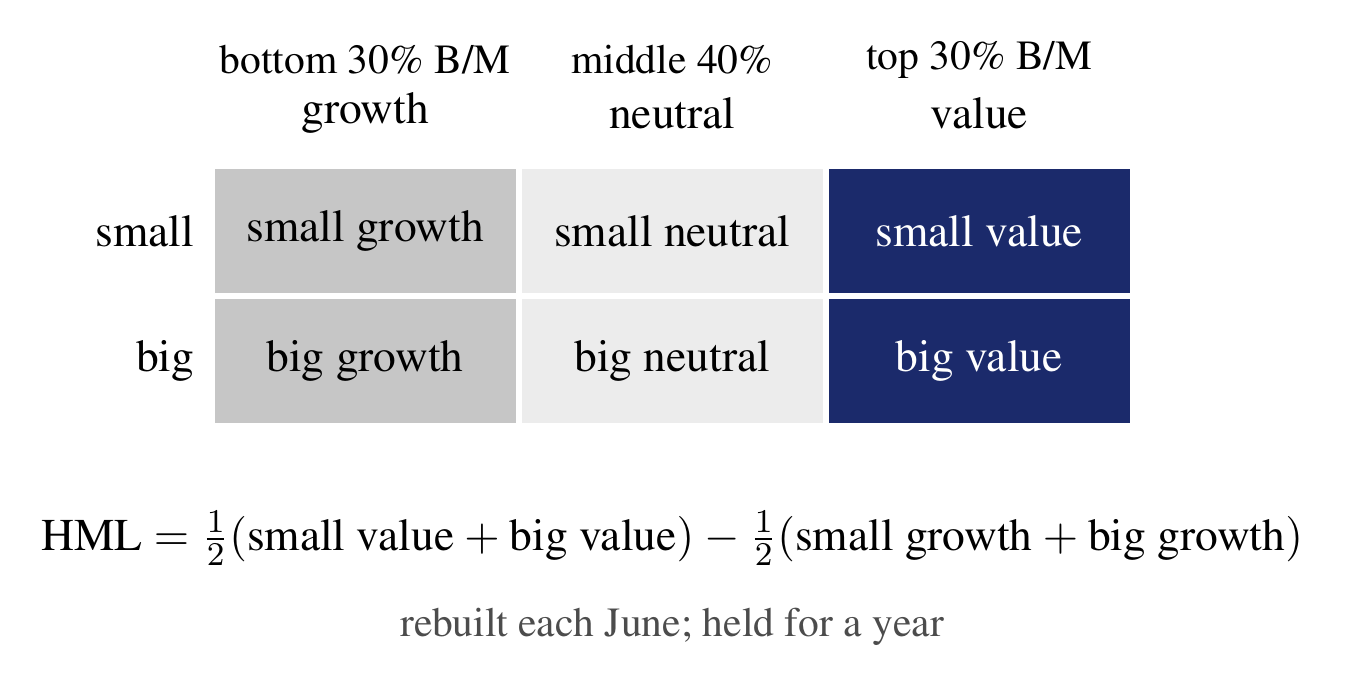
\includegraphics[width=0.85\linewidth]{images/fig08-2-hml.png}
\caption{How HML is built. Stocks are sorted into two size groups and three book-to-market groups. HML buys the two value portfolios and sells the two growth portfolios, so that small and big firms count equally.}
\label{fig:08-hml}
\end{figure}

The portfolios are held for a year and rebuilt the next June, using book equity from the fiscal year ending in the previous calendar year so that the accounting data would have been public (Section~\ref{sec:02-lookahead}). This design keeps HML's turnover low, about 3\% a month (Chapter 6; Novy-Marx and Velikov 2016).

\textbf{Why value might earn more.} Two families of explanation compete:

\begin{itemize}
  \item \textbf{Risk.} Value firms are often distressed or inflexible: they have assets in place that are hard to cut back in recessions. If they do worst in bad economic times, investors demand higher expected returns to hold them (Fama and French 1993; Zhang 2005).
  \item \textbf{Mispricing.} Investors extrapolate past growth too far into the future, overpaying for glamorous growth firms and shunning unexciting value firms. As the expected growth fails to arrive, prices correct (Lakonishok, Shleifer and Vishny 1994).
\end{itemize}

The distinction matters for the future. A risk premium should persist, though it may arrive unevenly. A mispricing can shrink as investors learn about it and as capital flows in to exploit it.

\section{The claim}
\label{sec:08-claim}

Stated so that it can fail:

\begin{callout}
\textbf{Stocks that are cheap relative to fundamentals earn higher average returns than expensive stocks, by enough to matter after costs, in data beyond the samples that established the result.}
\end{callout}

The last clause is the key. The value premium is well documented in the data that discovered it. The question is whether it held afterward, in other markets, with other measures, and at a size an investor could hold. Three tests follow from the claim:

\begin{itemize}
  \item \textbf{Time.} Does HML earn a positive premium after the original sample of Fama and French (1992), which ended in 1990, and in particular after 2007?
  \item \textbf{Breadth.} Does the premium appear with earnings, cash flow and dividends as well as book value, among large stocks as well as small ones, and in other countries?
  \item \textbf{Implementability.} Does it survive costs, and could an investor live with its \textbf{drawdowns}, the falls from a previous peak, long enough to collect it?
\end{itemize}

\section{The original evidence and its interpretations}
\label{sec:08-evidence}

\textbf{Before the factor.} Basu (1977) found that stocks with high earnings-to-price ratios earned higher risk-adjusted returns than the capital asset pricing model predicted. Rosenberg, Reid and Lanstein (1985) found the same for book-to-market. These were treated as anomalies: puzzles for the CAPM rather than a new principle.

\textbf{Fama and French (1992, 1993).} Using U.S. stocks from 1963 to 1990, Fama and French (1992) showed that size and book-to-market together captured the \textbf{cross-section of average returns}, the differences in average return across stocks, and that market beta, the CAPM's only variable, added nothing. Fama and French (1993) turned the finding into the three-factor model, with HML as the value factor, and interpreted it as compensation for a risk related to financial distress. The papers changed the field: the three-factor model became the standard benchmark for judging investment performance for two decades.

\textbf{Lakonishok, Shleifer and Vishny (1994)} offered the competing interpretation. Value stocks did not appear riskier in the ways that mattered: they did not do notably worse in bad markets or recessions. Instead, investors seemed to extrapolate past growth: \textbf{glamour} firms with strong past growth were priced as if it would continue, and it did not.

\textbf{Breadth.} Fama and French (1998) found value premiums in many international markets, and Asness, Moskowitz and Pedersen (2013) found value effects across countries and asset classes, from stocks to bonds to currencies to commodities. By the 2010s, value was one of the best-documented patterns in finance.

\textbf{The drought.} From 2007 to 2020, U.S. value stocks trailed growth stocks by a large cumulative margin, the longest and deepest drawdown in HML's history. Explanations multiplied.

\begin{itemize}
  \item \textbf{Mismeasured book value.} Book value had become a poor measure of a firm's assets because spending on research, software and brands is expensed rather than recorded as an asset. Eisfeldt, Kim and Papanikolaou (2022) showed that adding \textbf{capitalized} intangible investment, recorded as an asset rather than an expense, to book equity produced a value factor that performed substantially better, including in recent decades.
  \item \textbf{Interest rates and crowding.} Others pointed to falling interest rates, which raise the value of distant growth cash flows, or to crowding by investors following the same strategy.
  \item \textbf{Noise.} Fama and French (2021) split 1963--2019 in half and found much lower value premiums in the second half, especially among large stocks, but showed that the volatility of returns made it impossible to reject either that the premium was unchanged or that it had fallen to zero.
  \item \textbf{Revaluation.} Arnott, Harvey, Kalesnik and Linnainmaa (2021) argued that much of the drought reflected value stocks becoming cheaper relative to growth stocks, a revaluation that cannot continue indefinitely, rather than a disappearing premium.
\end{itemize}

\section{Replication lab: Lab 8}
\label{sec:08-lab}

\begin{callout}
\textbf{Lab 8 at a glance.} \emph{The question:} has HML earned a premium over the century of available U.S. data, and in particular since 2007? Does the answer depend on how cheapness is measured, on firm size, or on the country? \emph{Data:} Kenneth French's library: the Fama--French factors from July 1926; the six size and book-to-market portfolios; univariate portfolios formed on book-to-market, earnings-to-price, cash flow-to-price and dividend yield; and HML factors for North America, Europe, Japan, Asia Pacific ex Japan and the developed markets outside the United States, from 1990. Optionally, the Jensen--Kelly--Pedersen (2023) data extends the test to dozens of countries. \emph{Code:} repository folder \texttt{ch08-value/}, with a guided notebook.
\end{callout}

\textbf{The setup.}

\begin{itemize}
  \item \textbf{Part A, replication.} HML's average return, t-statistic, Sharpe ratio and CAPM alpha over the full sample and in four eras: 1926--1963, the original Fama--French sample of 1963--1990, 1991--2006, and 2007 to the present. A formal test asks whether the post-2007 premium differs from the earlier one by more than chance would allow.
  \item \textbf{Part B, stress tests.} Section~\ref{sec:08-stress} describes these.
  \item \textbf{Part C, other markets.} International HML before and after 2007.
  \item \textbf{Part D, living with value.} Drawdowns, the longest time spent below a previous peak, the worst ten-year period, and a bootstrap of ten-year outcomes used to size a value tilt (Section~\ref{sec:08-investors}).
\end{itemize}

\textbf{What readers will find.} Figure 8.3 shows the growth of a dollar in HML over the century, with the eras marked. Figure 8.4 sets out the premium in each era with its 95\% interval: the test of the claim over time is whether the post-2007 interval excludes the earlier premium, excludes zero, or neither. Fama and French's own split of 1963--2019 found the last of these, and readers can check whether the years since 2019 have changed the answer. Figure 8.7 shows how long value can disappoint, and Figure 8.8 turns that history into a range of ten-year outcomes.

\section{Stress tests}
\label{sec:08-stress}

\textbf{1. Other measures of cheapness.} If the value premium reflects something about cheap firms, it should appear whether cheapness is measured with book value, earnings, cash flow or dividends. If it appears only with book-to-market, it may be an artifact of accounting. The lab compares top-30\%-minus-bottom-30\% spreads for all four measures, over the full sample and before and after 2007. Book value is the measure most exposed to the intangibles problem, because research spending and brand building reduce book equity directly; earnings and cash flow are affected too, but less.

\textbf{2. Large stocks only.} Many anomalies are strongest among small stocks, which are expensive to trade and hold little of the market's value (Section~\ref{sec:02-microcaps}). The $2 \times 3$ portfolios separate value among big stocks from value among small stocks. Fama and French (2021) found that the decline in the second half of their sample was much larger for big stocks; the lab extends their comparison to the present.

\textbf{3. Intangible-adjusted book equity.} Eisfeldt, Kim and Papanikolaou (2022) capitalized research and development and a share of selling, general and administrative spending into book equity. Their intangible-adjusted value factor performed better throughout, including in the drought years. Replicating this requires firm-level accounting data that is not freely available, so the lab does not reproduce it; an exercise outlines how to do so with access to Compustat. Readers should note what the result implies: the drought was partly a measurement problem, not only a failure of the idea that cheap stocks earn more.

\textbf{4. After costs.} Value is a slow strategy. With turnover of about 3\% a month, a one-way trading cost of 20 to 50 basis points reduces its average return by roughly 0.3 to 0.7 percentage points a year (Equation~\eqref{eq:06-net}: $4 \times 0.03 \times 12 = 1.44$ times the one-way cost each year). Costs are not what threatens the value premium.

\textbf{5. Other countries.} If value works because of something general about how markets price cheap firms, it should appear outside the United States. The French international factors allow a test since 1990, before and after 2007. The Jensen--Kelly--Pedersen data, covering many more countries, also invites Chapter 4's warning: with dozens of countries, some will show significant premiums by chance, and some will show none.

\section{Verdict}
\label{sec:08-verdict}

Based on the published evidence through the end of the 2010s drought, to be confirmed by readers' runs of Lab 8 on data through 2025: \textbf{weakens.}

\begin{center}
\small
\begin{tabularx}{0.9\linewidth}{@{}>{\raggedright\arraybackslash}p{0.24\linewidth}>{\raggedright\arraybackslash}X>{\raggedright\arraybackslash}p{0.21\linewidth}@{}}
\toprule
Test & Finding & Effect on the claim \\
\midrule
Full century of U.S. data & HML earned a positive average premium, with a t-statistic well above conventional thresholds & Supports \\
After the original sample, and especially after 2007 & Much smaller, and for large U.S. stocks close to zero or negative over long stretches; statistically hard to distinguish either from the old premium or from zero & Weakens \\
Other measures of cheapness & The premium appears with earnings and cash flow as well as book value, though not identically & Supports breadth \\
Large stocks & Weaker than among small stocks, particularly in recent decades & Weakens \\
Intangible-adjusted book equity & A better-measured value factor performs better, including recently & Suggests part of the drought is mismeasurement \\
Other countries & Present in many markets, but uneven across countries and periods & Supports, with variation \\
Costs & Small relative to the premium & No effect \\
\bottomrule
\end{tabularx}
\end{center}

The claim that cheap stocks earn more than expensive ones has a century of support and a sound economic logic, but its size, its reliability and the measure of cheapness that captures it are all less certain than the field believed in the 1990s. The verdict is dated by the sample tested; a value premium that returned strongly for a decade would move it toward survives, and another decade like 2007--2020 toward fails.

\section{What investors can use}
\label{sec:08-investors}

The central lesson of value's history is not about its average return but about its patience requirement.

\textbf{Size the tilt you can hold through ten bad years.} A \textbf{value tilt} of weight $w$ adds $w$ times HML to a market portfolio, so its return relative to the market is $w$ times HML. Lab 8's Part D resamples HML's history to estimate a bad-case ten-year outcome, the 5th percentile, and reports the largest tilt whose bad case stays within a shortfall you specify. An investor who would abandon a strategy after trailing the market by 10\% over a decade should hold no larger a tilt than that, because abandoning it after the losses and before the recovery is the worst outcome of all.

\textbf{Expect long droughts.} Even if the premium is real, the lab's drawdown statistics show how long HML can spend below a previous peak. A premium that arrives once a decade, irregularly, is a premium most investors will not stay to collect.

\textbf{Prefer measures that are harder to distort.} Composite measures that combine several value signals, and book equity adjusted for intangible investment, are less exposed to accounting changes than raw book-to-market.

\textbf{Questions to ask a value manager:}

\begin{enumerate}
  \item Which measure of cheapness do you use, and how did it perform from 2007 to 2020?
  \item How much of your historical return comes from small stocks you could not hold at your current size?
  \item How do you handle firms whose book value omits most of their assets, such as software, pharmaceutical and brand-driven companies?
  \item What is your worst ten-year relative performance in your backtest and in live trading, and how did clients respond?
  \item Is your recent improvement a return of the premium, or value stocks becoming more expensive relative to growth?
\end{enumerate}

\begin{callout}
\textbf{What Failed: confident calls on value's death and its return.} As the drought deepened in the late 2010s, confident claims multiplied in both directions. Some declared value permanently dead, arbitraged away by the factor-investing industry or made obsolete by a technology-driven economy. Others declared, year after year, that a sharp comeback was imminent because value had become historically cheap relative to growth. Both claims ran ahead of the evidence. A premium whose year-to-year volatility is large relative to its average cannot be declared dead after a decade of losses, as Fama and French (2021) showed formally; and cheapness relative to growth, while it raises expected returns, says little about when they will arrive. Value rebounded strongly in 2021 and 2022 and then lagged again. The claim that anyone could confidently time value's death or its revival \textbf{fails}.
\end{callout}

\section{Open questions}
\label{sec:08-open}

\begin{itemize}
  \item \textbf{Has intangible investment changed what ``cheap'' means?} If so, what is the right measure of a firm's invested capital, and does a properly measured value premium look stable?
  \item \textbf{Risk or mispricing?} The drought is a natural experiment. Did value's losses coincide with bad times for investors, as a risk story would require, or with good times?
  \item \textbf{Interest rates.} How much of value's performance since 2007 is explained by falling, then rising, interest rates acting on the long-duration cash flows of growth firms?
  \item \textbf{International divergence.} Why has the value premium been more persistent in some markets, such as Japan, than in the United States?
  \item \textbf{Crowding.} Did the growth of value funds and factor products reduce the premium, and can crowding be measured in advance?
\end{itemize}

\section*{Exercises}
\addcontentsline{toc}{section}{Exercises}

\subsection*{Conceptual (all readers)}

\begin{enumerate}
  \item Explain the difference between the risk and mispricing explanations of the value premium. What evidence from the 2007--2020 drought would favor each?
  \item Why does HML use book equity from the previous fiscal year and rebalance only in June? What would go wrong with monthly rebalancing on the latest accounting data?
  \item A firm spends heavily on research and development. How does that spending affect its book-to-market ratio, and why might it be misclassified as a growth stock?
  \item Explain why a value premium of 4\% a year with 12\% annual volatility cannot be distinguished from zero over a 15-year period. How many years would be needed?
\end{enumerate}

\subsection*{Lab extensions (technical readers)}

\begin{enumerate}
  \setcounter{enumi}{4}
  \item Split the sample at 1990 instead of 2007. Which break looks more like a change in the premium?
  \item Compare value among large and small stocks after 2007. What does the comparison imply about who could actually have earned the premium?
  \item Run Part D with a tolerance of 5\% and 20\%. How does the largest tilt change, and what would you recommend to a cautious and to a patient investor?
  \item With the JKP data, count the countries in which the value premium has a t-statistic above 2. How many would you expect by chance?
  \item With access to firm-level accounting data, rebuild book equity by capitalizing research and development and part of selling, general and administrative spending, and rebuild HML. Does the post-2007 shortfall shrink?
  \item Measure the \textbf{value spread}, the gap in book-to-market between value and growth portfolios, over time. Does a wide spread predict higher subsequent HML returns? Apply Chapter 5's out-of-sample tests.
\end{enumerate}

\section*{References}
\addcontentsline{toc}{section}{References}

\begin{itemize}
  \item Arnott, R. D., Harvey, C. R., Kalesnik, V. and Linnainmaa, J. T. (2021). Reports of Value's Death May Be Greatly Exaggerated. \emph{Financial Analysts Journal} 77(1): 44--67.
  \item Asness, C. S., Moskowitz, T. J. and Pedersen, L. H. (2013). Value and Momentum Everywhere. \emph{Journal of Finance} 68(3): 929--985.
  \item Basu, S. (1977). Investment Performance of Common Stocks in Relation to Their Price-Earnings Ratios: A Test of the Efficient Market Hypothesis. \emph{Journal of Finance} 32(3): 663--682.
  \item Eisfeldt, A. L., Kim, E. T. and Papanikolaou, D. (2022). Intangible Value. \emph{Critical Finance Review} 11(2): 299--332.
  \item Fama, E. F. and French, K. R. (1992). The Cross-Section of Expected Stock Returns. \emph{Journal of Finance} 47(2): 427--465.
  \item Fama, E. F. and French, K. R. (1993). Common Risk Factors in the Returns on Stocks and Bonds. \emph{Journal of Financial Economics} 33(1): 3--56.
  \item Fama, E. F. and French, K. R. (1998). Value versus Growth: The International Evidence. \emph{Journal of Finance} 53(6): 1975--1999.
  \item Fama, E. F. and French, K. R. (2021). The Value Premium. \emph{Review of Asset Pricing Studies} 11(1): 105--121.
  \item Graham, B. and Dodd, D. L. (1934). \emph{Security Analysis}. New York: McGraw-Hill.
  \item Jensen, T. I., Kelly, B. and Pedersen, L. H. (2023). Is There a Replication Crisis in Finance? \emph{Journal of Finance} 78(5): 2465--2518.
  \item Lakonishok, J., Shleifer, A. and Vishny, R. W. (1994). Contrarian Investment, Extrapolation, and Risk. \emph{Journal of Finance} 49(5): 1541--1578.
  \item Novy-Marx, R. and Velikov, M. (2016). A Taxonomy of Anomalies and Their Trading Costs. \emph{Review of Financial Studies} 29(1): 104--147.
  \item Rosenberg, B., Reid, K. and Lanstein, R. (1985). Persuasive Evidence of Market Inefficiency. \emph{Journal of Portfolio Management} 11(3): 9--16.
  \item Zhang, L. (2005). The Value Premium. \emph{Journal of Finance} 60(1): 67--103.
\end{itemize}

\textbf{Data:} Kenneth R. French Data Library, \url{https://mba.tuck.dartmouth.edu/pages/faculty/ken.french/data_library.html}. Jensen--Kelly--Pedersen global factor data, \url{https://jkpfactors.com}.
